\iffalse
                       
                        
                        
                        
                    
                        \author{AI24BTECH11006 - Bugada Roopansha}
                        \section{PH}
                        \chapter{2018}
                        \fi
 
   \item The eigenvalues of a Hermitian matrix are all
   \begin{enumerate}
       \item real
\item imaginary
\item of modulus one
\item  real and positive
   \end{enumerate}


\item Which one of the following represents the $3p$ radial wave function of the hydrogen atom? $\brak{a_0 \text{ is the Bohr radius}}$

\begin{enumerate}

\item
\begin{center}
    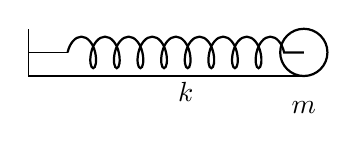
\begin{tikzpicture}
        % Drawing the spring
        \draw[thick, decoration={coil,aspect=0.5,segment length=3mm, amplitude=2mm}, decorate] (0,0) -- (3,0);
        \node at (1.5,-0.5) {$k$};

        % Drawing the disc
        \draw[thick] (3,0) circle (0.3);
        \node at (3,-0.7) {$m$};

        \draw (-0.5,-0.3) -- (3,-0.3);
        \draw (-0.5,0) -- (0,0);
        \draw (-0.5,-0.3) -- (-0.5,0.3);
    \end{tikzpicture}
    \end{center}


\item
\begin{center}
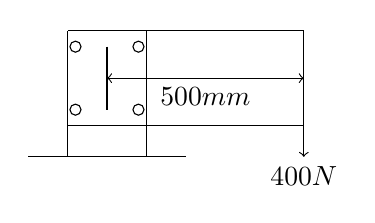
\begin{tikzpicture}
    % Draw rivets as circles
    \draw (0.4, 0.4) circle (2pt) node[above right] {};
    \draw (0.4, -0.4) circle (2pt) node[below right] {};
    \draw (-0.4, 0.4) circle (2pt) node[above left] {};
    \draw (-0.4, -0.4) circle (2pt) node[below left] {};

    

    % Draw horizontal and vertical distances between rivets
    \draw (0.5, 0.6) -- (-0.5, 0.6) ;
    \draw (0.5, -0.6) -- (-0.5, -0.6);
    \draw (-0.5, -0.6) -- (-0.5,0.6);
    \draw (0.5, -0.6) -- (0.5, 0.6);
    \draw (0.5, -0.6) -- (0.5, -1);
    \draw (-0.5, -0.6) -- (-0.5, -1);
   \draw (1, -1) -- (-1, -1);
    \draw (0.5, 0.6) -- (2.5, 0.6) ;
    \draw (0.5, -0.6) -- (2.5, -0.6) ;
    \draw (2.5 ,0.6) -- (2.5 ,-0.6);
    \draw[->] (2.5,-0.6) -- (2.5 ,-1) node[below]{$400N$} ;
    \draw (0,0.4) -- (0,-0.4);
    \draw[<->] (0,0) -- (2.5,0) node[below,midway]{$500 mm$};
\end{tikzpicture}
\end{center}

\item
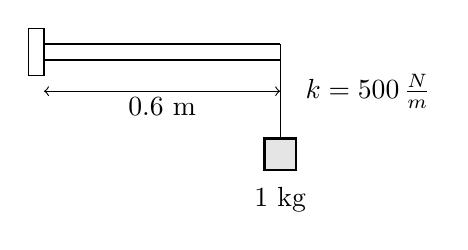
\begin{tikzpicture}
    % Draw the main beam
    \draw[thick] (0,0) -- (3,0);
    \draw[thick] (0,-0.2) -- (3,-0.2);
    
    % Add end support
    \draw (-0.2,-0.4) rectangle (0,0.2);
    
    % Add dimension line and label
    \draw[<->] (0,-0.6) -- (3,-0.6);
    \node at (1.5,-0.8) {0.6 m};
    
    % Draw spring
    \draw (3,0) -- (3, -1.2);
    \node[anchor=west] at (3.2, -0.6) {$k=500\,\frac{N}{m}$};
    
    % Draw mass
    \fill[gray!20] (2.8, -1.6) rectangle (3.2, -1.2);
    \draw[thick] (2.8, -1.6) rectangle (3.2, -1.2);
    \node[anchor=north] at (3, -1.7) {1 kg};
    
    \end{tikzpicture}

\item
\begin{tikzpicture}[scale=0.6] % Adjust the scale factor as needed
    % Axes
    \draw[->] (-1,0) -- (6,0) node[right] {$r/a_0$};
    \draw[->] (0,-1) -- (0,4) node[above] {R(r)};

    % Bézier curve from (0,0) to (5,3) with control points
    \draw[thick, color=black]
        (0,0) .. controls (0.5,5) and (1,-0.5) .. (3,0.1);

    % Mark point
    \fill (0,0) circle (2pt) node[below left] { O};
\end{tikzpicture}


\end{enumerate}



\item Given the following table,

\begin{center}
        \begin{center}
    \begin{tabular}{|p{3cm}|p{3cm}|}
        \hline
        \textbf{Machining Process} & \textbf{Mechanism of Material Removal} \\
        \hline
        P. Chemical machining & $1.$ Erosion \\
        Q. Electro-chemical machining & $2.$ Corrosive reaction \\
        R. Electro-discharge machining & $3.$ Ion displacement \\
        S. Ultrasonic machining & $4.$ Fusion and vaporization \\
        \hline
    \end{tabular}
\end{center}

Which one of the following correctly matches the experiments from Group I to their inferences in Group II?
\begin{enumerate}
    \item P-$2$, Q-$3$, R-$4$, S-$1$
    \item P-$1$, Q-$3$, R-$2$, S-$4$
    \item P-$3$, Q-$4$, R-$2$, S-$1$
    \item P-$2$, Q-$1$, R-$4$, S-$3$
\end{enumerate}

\item In spherical polar coordinates $ \brak{r, \theta, \phi} $, the unit vector $\hat{\theta}$ at $\brak{10, \frac{\pi}{4}, \frac{\pi}{2}}$ is
\begin{enumerate}
    \item $\hat{k}$
    \item $\frac{1}{\sqrt{2}} \brak{\hat{j} + \hat{k}}$
    \item $\frac{1}{\sqrt{2}} \brak{-\hat{j} + \hat{k}}$
    \item $\frac{1}{\sqrt{2}} \brak{\hat{j} - \hat{k}}$
\end{enumerate}

\item The scale factors corresponding to the covariant metric tensor $g$ in spherical polar coordinates are
\begin{enumerate}
    \item $1, r^2, r^2 \sin^2 \theta$
    \item $1, r^2, \sin^2 \theta$
    \item $1, 1, 1$
    \item $1, r, r \sin \theta$
\end{enumerate}

\item In the context of small oscillations, which one of the following does NOT apply to the normal coordinates?
\begin{enumerate}
    \item Each normal coordinate has an eigen-frequency associated with it
    \item The normal coordinates are orthogonal to one another
    \item The normal coordinates are all independent
    \item The potential energy of the system is a sum of squares of the normal coordinates with constant coefficients
\end{enumerate}

\item For the given unit cells of a two-dimensional square lattice, which option lists all the primitive cells?\\
\begin{tikzpicture}
    % Axes
    \draw[thick,->] (0,0) -- (4,0) node[right] {$S$};
    \draw[thick,->] (0,0) -- (0,4) node[above] {$T$};
    
    % Labels for points
    \node[right] at (3,3) {$1$};
    \node[left] at (1,1) {$2$};
    \node[left] at (2,3) {$3$};
    
    % Curves
    \draw (2,3) to (3,3);
    \draw (1,1) parabola (3,3);
    \draw (1,1) parabola (2,3);
    
   
\end{tikzpicture}

\begin{enumerate}
    \item $1$ and $2$
    \item $1$,$2$ and $3$
  \item $1$,$2$,$3$ and $4$
   \item  $1$,$2$,$3$,$4$ and $5$
\end{enumerate}

\item Among electric field $\brak{\vec{E}}$, magnetic field $\brak{\vec{B}}$, angular momentum $\brak{\vec{L}}$, and vector potential $\brak{\vec{A}}$, which is/are odd under parity \brak{\text{space inversion}} operation?
\begin{enumerate}
    \item $\vec{E}$ only
    \item $\vec{E}$ \& $\vec{A}$ only
    \item $\vec{E}$ \& $\vec{B}$ only
    \item $\vec{B}$ \& $\vec{L}$ only
\end{enumerate}

\item The expression for the second overtone frequency in the vibrational absorption spectra of a diatomic molecule in terms of the harmonic frequency $\omega$ and anharmonicity constant $x_e$, is
\begin{enumerate}
    \item $2 \omega_e \brak{1 - x_e}$
    \item $2 \omega_e \brak{1 - 3x_e}$
    \item $3 \omega_e \brak{1 - 2x_e}$
    \item $3 \omega_e \brak{1 - 4x_e}$
\end{enumerate}

\item Match the physical effects and order of magnitude of their energy scales given below, where $\alpha=\frac{e^2}{4\pi\epsilon_o\hbar c}$ is the fine structure constant, $m_e$ and $m_p$ are the electron and proton masses, respectively.

\begin{tabular}{|c|c|}
\hline
Group I & Group II \\ \hline
P: Lamb shift & $1: \sim 0 \brak{\alpha^2 m_e c^2}$ \\ \hline
Q: Fine structure & $2: \sim 0 \brak{\alpha^4 m_e c^2}$ \\ \hline
R: Bohr energy & $3: \sim 0 \brak{\frac{\alpha^4 m_e^2 c^2}{ m_p}}$ \\ \hline
S: Hyperfine structure & $4: \sim 0 \brak{\alpha^5 m_p c^2}$ \\ \hline
\end{tabular}


\begin{enumerate}
    \item $P-3, Q-1, R-2, S-4$
    \item $P-2, Q-3, R-1, S-4$
    \item $P-4, Q-2, R-1, S-3$
    \item $P-2, Q-4, R-1, S-3$
\end{enumerate}

\item The logic expression $\bar{A}BC + \bar{A}\bar{B}C + AB\bar{C} + A\bar{B}\bar{C}$ can be simplified to
\begin{enumerate}
    \item $A XOR C$
    \item $A AND C$
    \item $0$
    \item $1$
\end{enumerate}

\item At low temperatures $\brak{T}$, the specific heat of common metals is described by $\brak{\text{with} \alpha \text{and} \beta \text{as constants}}$
\begin{enumerate}
    \item $\alpha T + \beta T^3$
    \item $\beta T^3$
    \item $\exp\brak{-\frac{\alpha}{T}}$
    \item $\alpha T + \beta T^5$
\end{enumerate}

\item In a $2$-to-$1$ multiplexer as shown below, the output $X=A_0$ if $C=0$ and $X=A_1$ if $C=1$.\\
\begin{figure}[!ht]
\centering
\resizebox{0.3\textwidth}{!}{%
\begin{circuitikz}
\tikzstyle{every node}=[font=\LARGE]
\draw (7.75,8) to[short] (7.75,8);
\draw (7.75,7.5) to[short] (7.75,7.5);

\node [font=\Large] at (14,8.5) {};
\node [font=\Large] at (14,8.5) {};
\draw  (10.25,9) rectangle (11.75,7);

\draw (11.75,8) to[short] (13,8);
\draw (11,10) to[short] (11,9);
\draw (9,8.25) to[short] (10.25,8.25);
\draw (9,7.5) to[short] (10.25,7.5);
\node [font=\LARGE] at (11,10.25) {C};
\node [font=\LARGE] at (13.5,8) {X};
\node [font=\LARGE] at (8.5,8) {$A_0$};
\node [font=\LARGE] at (8.5,7.5) {$A_1$};
\end{circuitikz}
}%
\end{figure}

Which one of the following is the correct implementation of this multiplexer?
\begin{enumerate}
    \item 
\begin{tikzpicture}

% Define coordinates for reference points
\coordinate (P) at (0,0,0);  % Point P
\coordinate (top) at (0,3,0);  % Top of the vertical segment
\coordinate (end) at (5,3,0);  % End of the horizontal segment
\coordinate (base1) at (-2,-0.5,-2);  % Base corners


% Draw the base plate
\draw[thick] (base1) -- ++(0,0,4) -- ++(4,0,0) -- ++(0,0,-4) -- cycle;


% Draw the vertical segment (pipe)


% Draw the horizontal segment (pipe)


% Draw the 600 N force at the end of the pipe

% Labels and dimensions
\draw (-0.5,0,0) -- (-0.5,5,0);
\draw (0.5,0,0) -- (0.5,4.5,0);
\draw (6,5,0) -- (-0.5,5,0);
\draw (6,4.5,0) -- (0.5,4.5,0);
\draw (6,5.5,0) -- (-0.5,5.5,0) node[above,midway] {500mm};
\draw (-1,0,0) -- (-1,5,0)node[left,midway] {300mm};
\draw[->] (P) -- ++(0,7,0) node[above] {$y$};  % y-axis
\draw[->] (P) -- ++(5,0,0) node[right] {$x$};  % x-axis
\draw[->] (P) -- ++(0,0,4) node[below] {$z$};  % z-axis


% Label point P
\node at (-0.2,-0.2) {P};

\end{tikzpicture}


\item 
\centering
\resizebox{0.3\textwidth}{!}{%  % Set to 50% of the text width
\begin{circuitikz}
\tikzstyle{every node}=[font=\LARGE]
% Connections for the first AND gate
\draw (5.5,9.75) to[short] (7.5,9.75);
\draw (7.5,9.75) to[short] (7.75,9.75);
\draw (7.5,9.25) to[short] (7.75,9.25);
\draw (7.75,9.75) node[ieeestd and port, anchor=in 1, scale=0.89](port1){} (port1.out) to[short] (9.5,9.5);

% Connections for other components
\draw (5.75,8) to[short] (5.75,9.25);
\draw (4.5,8.5) to[short] (5.75,8.5);
\draw (7.75,8) to[short] (7.75,8);
\draw (7.75,7.5) to[short] (7.75,7.5);
\draw (7.75,8) node[ieeestd and port, anchor=in 1, scale=0.89](port2){} (port2.out) to[short] (9.5,7.75);
\draw (6.5,7.5) to[short] (7.75,7.5);

% OR gate connections
\draw (9.5,9.5) to[short] (9.5,8.75);
\draw (9.5,8.25) to[short] (11.5,8.25);
\draw (9.5,8.75) to[short] (11.5,8.75);
\draw (9.5,7.75) to[short] (9.5,8.25);
\draw (11.25,8.75) to[short] (11.5,8.75);
\draw (11.25,8.25) to[short] (11.5,8.25);
\draw (11.5,8.75) node[ieeestd or port, anchor=in 1, scale=0.89](port3){} (port3.out) to[short] (13.25,8.5);

% Output node and labels
\node at (13.25,8.5) [circ] {};
\node [font=\Large] at (14,8.5) {X};

% Input labels
\node [font=\Large] at (5,9.5) {$A_0$};
\node [font=\Large] at (4,8.5) {C};
\node [font=\Large] at (6,7.5) {$A_1$};

% Additional short connections for clarity
\draw (7.5,9.25) to[short] (5.75,9.25);
\draw (7.5,8) to[short] (7.75,8);
\draw (7.5,7.5) to[short] (7.75,7.5);
\draw (5.75,8) to[short, -o] (7.75,8);

\end{circuitikz}
}%


\item 


\resizebox{0.3\textwidth}{!}{
\begin{circuitikz}
\tikzstyle{every node}=[font=\LARGE]
\draw (5.5,9.75) to[short] (7.5,9.75);
\draw (5.75,8) to[short] (5.75,9.25);
\draw (4.5,8.5) to[short] (5.75,8.5);
\draw (7.75,8) to[short] (7.75,8);
\draw (7.75,7.5) to[short] (7.75,7.5);
\draw (7.75,8) node[ieeestd and port, anchor=in 1, scale=0.89](port1){} (port1.out) to[short] (9.5,7.75);
\draw (6.5,7.5) to[short] (7.75,7.5);
\draw (9.5,9.5) to[short] (9.5,8.75);
\draw (9.5,8.25) to[short] (11.5,8.25);
\draw (9.5,8.75) to[short] (11.5,8.75);
\draw (9.5,7.75) to[short] (9.5,8.25);
\draw (11.25,8.75) to[short] (11.5,8.75);
\draw (11.25,8.25) to[short] (11.5,8.25);
\draw (11.5,8.75) node[ieeestd or port, anchor=in 1, scale=0.89](port2){} (port2.out) to[short] (13.25,8.5);

% Output node and labels
\node at (13.25,8.5) [circ] {};
\node [font=\Large] at (14,8.5) {X};

% Input labels
\node [font=\Large] at (5,9.5) {$A_0$};
\node [font=\Large] at (4,8.5) {C};
\node [font=\Large] at (6,7.5) {$A_1$};

% Additional connections
\draw (7.5,8) to[short] (5.75,8);
\draw (7.5,8) to[short] (7.75,8);
\draw (7.5,7.5) to[short] (7.75,7.5);
\draw (7.5,9.75) to[short] (7.75,9.75);
\draw (7.5,9.25) to[short] (7.75,9.25);
\draw (7.75,9.75) node[ieeestd or port, anchor=in 1, scale=0.89](port4){} (port4.out) to[short] (9.5,9.5);
\draw (5.75,9.25) to[short, -o] (7.75,9.25);
\end{circuitikz}
}%


\item 



\resizebox{0.3\textwidth}{!}{%  % Set to 60% of the text width
\begin{circuitikz}
\tikzstyle{every node}=[font=\LARGE]
\draw (5.5,9.75) to[short] (7.5,9.75);
\draw (7.5,9.75) to[short] (7.75,9.75);
\draw (7.5,9.25) to[short] (7.75,9.25);
\draw (7.75,9.75) node[ieeestd and port, anchor=in 1, scale=0.89](port1){} (port1.out) to[short] (9.5,9.5);
\draw (5.75,8) to[short] (5.75,9.25);
\draw (4.5,8.5) to[short] (5.75,8.5);
\draw (7.75,8) to[short] (7.75,8);
\draw (7.75,7.5) to[short] (7.75,7.5);
\draw (7.75,8) node[ieeestd and port, anchor=in 1, scale=0.89](port2){} (port2.out) to[short] (9.5,7.75);
\draw (6.5,7.5) to[short] (7.75,7.5);
\draw (9.5,9.5) to[short] (9.5,8.75);
\draw (9.5,8.25) to[short] (11.5,8.25);
\draw (9.5,8.75) to[short] (11.5,8.75);
\draw (9.5,7.75) to[short] (9.5,8.25);
\draw (11.25,8.75) to[short] (11.5,8.75);
\draw (11.25,8.25) to[short] (11.5,8.25);
\draw (11.5,8.75) node[ieeestd or port, anchor=in 1, scale=0.89](port3){} (port3.out) to[short] (13.25,8.5);

% Output node and labels
\node at (13.25,8.5) [circ] {};
\node [font=\Large] at (14,8.5) {X};

% Input labels
\node [font=\Large] at (5,9.5) {$A_0$};
\node [font=\Large] at (4,8.5) {C};
\node [font=\Large] at (6,7.5) {$A_1$};

% Additional connections
\draw (7.5,9.25) to[short] (5.75,9.25);
\draw (7.5,8) to[short] (5.75,8);

\end{circuitikz}
}%



\end{enumerate}

                                        




